%!TeX program = lualatex
\renewcommand{\thelektion}{L10 \textperiodcentered{} Aufbau eines Computers I}

\begin{frame}\lessontitle{Lektion 10}{Aufbau eines Computers I}{Von-Neumann-Architektur \& die CPU im Detail \textperiodcentered{} Skript, Kapitel 5}\end{frame}

\begin{frame}\FDUtitle{Vom Gatter zum Computer}
\begin{center}
Wir kennen jetzt Gatter und den Halbaddierer.
\vspace{4mm}

Wie setzt man daraus einen \textbf{vollständigen Computer} zusammen?
\end{center}
\begin{center}
\begin{tikzpicture}[node distance=1.5cm]
    \node[draw, fill=RoyalBlue!15, minimum width=2.5cm, minimum height=1cm, rounded corners] (ein) {Eingabe};
    \node[draw, fill=Goldenrod!30, minimum width=2.5cm, minimum height=1cm, rounded corners, right=of ein] (ver) {Verarbeitung};
    \node[draw, fill=DarkSeaGreen!40, minimum width=2.5cm, minimum height=1cm, rounded corners, right=of ver] (aus) {Ausgabe};
    \draw[->, thick] (ein) -- (ver);
    \draw[->, thick] (ver) -- (aus);
\end{tikzpicture}

\end{center}
\end{frame}

{\setbeamertemplate{footline}{\darkfootline}
\begin{frame}\sectionframe[FDUblue]{Die Von-Neumann-Architektur}{1945, John von Neumann}
\end{frame}}

\begin{frame}\FDUtitle{Das entscheidende Merkmal}
\begin{center}
\textbf{Programm und Daten} liegen im \textbf{gleichen} Speicher.
\vspace{4mm}

Das Programm ist selbst nur ein Stück Daten -- also eine Bitfolge, die jederzeit verändert oder ausgetauscht werden kann.
\end{center}
\end{frame}

\begin{frame}\FDUtitle{Die Hauptkomponenten}
\begin{center}
\input{Grundlagen_Info/16_ComputerUndKodierungen/Figures/tikz_von_neumann.tex}
\end{center}
\end{frame}

\begin{frame}\FDUtitle{Die Büro-Analogie (mentales Modell)}
\begin{center}
\scalebox{0.82}{
\begin{tabular}{lll}
    \textbf{Komponente} & \textbf{Rolle im Büro} & \textbf{Eigenschaft} \\\midrule
    \textbf{CPU} & \textbf{Arbeitende Person} & Rechnet und führt Befehle aus \\
    \quad $\hookrightarrow$ \textit{Steuerwerk} & Gehirn / Planer (liest Anleitung) & Steuert Ablauf und Takt \\
    \quad $\hookrightarrow$ \textit{ALU} & Taschenrechner / Werkzeug & Arithmetik und Vergleiche \\
    \quad $\hookrightarrow$ \textit{Register} & Notizblock / Hände & Winzig, extrem schnell \\
    \textbf{RAM} & \textbf{Schreibtischplatte} & Schnell; am Feierabend leer (\emph{flüchtig}) \\
    \textbf{Massenspeicher} & \textbf{Aktenschrank / Archiv} & Dauerhaft (\emph{nicht flüchtig}), langsamer \\
    \textbf{Systembus} & \textbf{Laufwege / Förderband} & Verbindet alle Bauteile \\
    \textbf{Ein-/Ausgabe} & \textbf{Posteingang \& Fenster} & Schnittstelle zur Aussenwelt \\
\end{tabular}}
\end{center}
\end{frame}

\begin{frame}\FDUtitle{Hauptplatine (Mainboard)}
\begin{center}
\resizebox{0.82\textwidth}{!}{%
\providecommand{\mainboardHighlight}{all}

\tikzset{
    mbActive/.style={opacity=1.0, text opacity=1.0},
    mbDimmed/.style={opacity=0.18, text opacity=0.22}
}

\newcommand{\mbSetScope}[1]{%
    \tikzset{mbScope/.style={mbDimmed}}%
    \edef\mbCurVal{#1}%
    \edef\mbHLVal{\mainboardHighlight}%
    \ifx\mbHLVal\mbCurVal
        \tikzset{mbScope/.style={mbActive}}%
    \else
        \def\mbAllVal{all}%
        \ifx\mbHLVal\mbAllVal
            \tikzset{mbScope/.style={mbActive}}%
        \else
            \def\mbStorageVal{storage}\def\mbSSDVal{ssd}%
            \ifx\mbHLVal\mbStorageVal\ifx\mbCurVal\mbSSDVal\tikzset{mbScope/.style={mbActive}}\fi\fi
            \ifx\mbHLVal\mbSSDVal\ifx\mbCurVal\mbStorageVal\tikzset{mbScope/.style={mbActive}}\fi\fi
            \def\mbPCIeVal{pcie}\def\mbSlotsVal{slots}\def\mbBusVal{bus}%
            \ifx\mbHLVal\mbPCIeVal\ifx\mbCurVal\mbSlotsVal\tikzset{mbScope/.style={mbActive}}\fi\fi
            \ifx\mbHLVal\mbPCIeVal\ifx\mbCurVal\mbBusVal\tikzset{mbScope/.style={mbActive}}\fi\fi
            \ifx\mbHLVal\mbSlotsVal\ifx\mbCurVal\mbPCIeVal\tikzset{mbScope/.style={mbActive}}\fi\fi
            \ifx\mbHLVal\mbBusVal\ifx\mbCurVal\mbPCIeVal\tikzset{mbScope/.style={mbActive}}\fi\fi
            \ifx\mbHLVal\mbBusVal\ifx\mbCurVal\mbSlotsVal\tikzset{mbScope/.style={mbActive}}\fi\fi
        \fi
    \fi
}

\begin{tikzpicture}[
    scale=0.88,
    every node/.style={transform shape},
    board/.style={fill=DarkSlateGray!12, draw=DarkSlateGray!80, line width=1.4pt, rounded corners=6pt},
    trace/.style={draw=RoyalBlue!80, line width=1.2pt},
    buslabel/.style={font=\scriptsize\bfseries\sffamily, text=RoyalBlue!90!black, fill=white, inner sep=1.5pt, rounded corners=2pt}
]
    % --- Mainboard Platine ---
    \def\mbAllVal{all}%
    \edef\mbHLVal{\mainboardHighlight}%
    \ifx\mbHLVal\mbAllVal
        \tikzset{mbBoardScope/.style={opacity=1.0, text opacity=1.0}}%
    \else
        \tikzset{mbBoardScope/.style={opacity=0.45, text opacity=0.55}}%
    \fi
    \begin{scope}[mbBoardScope]
        \draw[board] (-6.3, -4.2) rectangle (6.3, 4.2);
        \node[anchor=north west, font=\bfseries\sffamily\footnotesize, text=DarkSlateGray!80] at (-4.2, 4.0) {Hauptplatine (Mainboard)};
    \end{scope}

    % --- I/O Panel (links) ---
    \mbSetScope{io}
    \begin{scope}[mbScope]
        \draw[fill=Salmon!25, draw=Salmon!90!black, line width=1pt, rounded corners=2pt] (-6.1, 0.4) rectangle (-4.8, 3.4);
        \node[rotate=90, font=\bfseries\sffamily\scriptsize, text=Salmon!90!black] at (-5.45, 1.9) {I/O-Panel};
        \foreach \y in {0.8, 1.5, 2.2, 2.9} {
            \draw[fill=gray!60, draw=black!70] (-6.2, \y-0.2) rectangle (-5.9, \y+0.2);
        }
        \node[anchor=east, font=\tiny\sffamily, text=black!75, align=right] at (-6.25, 1.9) {Tastatur/Maus\\Monitor / LAN};
    \end{scope}

    % --- CPU Sockel & Prozessor (Mitte-Links) ---
    \mbSetScope{cpu}
    \begin{scope}[mbScope]
        \draw[fill=ForestGreen!15, draw=ForestGreen!80!black, line width=1.4pt, rounded corners=4pt] (-3.9, 0.4) rectangle (-0.5, 3.4);
        \node[anchor=north, font=\bfseries\sffamily\footnotesize, text=ForestGreen!90!black] at (-2.2, 3.35) {CPU-Sockel};

        % CPU Innenleben (ALU, Register, Steuerwerk)
        \draw[fill=ForestGreen!30, draw=ForestGreen!90!black, line width=1pt, rounded corners=3pt] (-3.6, 0.6) rectangle (-0.8, 2.8);
        
        % Sub-blocks
        \draw[fill=ForestGreen!60, draw=ForestGreen!90!black, rounded corners=1.5pt] (-3.4, 1.8) rectangle (-2.7, 2.5);
        \node[font=\tiny\bfseries\sffamily, text=white] at (-3.05, 2.15) {ALU};
        
        \draw[fill=Gray!60, draw=Gray!90!black, rounded corners=1.5pt] (-2.55, 1.8) rectangle (-1.85, 2.5);
        \node[font=\tiny\bfseries\sffamily, text=white] at (-2.2, 2.15) {Reg};
        
        \draw[fill=RoyalBlue!60, draw=RoyalBlue!90!black, rounded corners=1.5pt] (-1.7, 1.8) rectangle (-1.0, 2.5);
        \node[font=\tiny\bfseries\sffamily, text=white] at (-1.35, 2.15) {Ctrl};
        
        \node[font=\tiny\sffamily\bfseries, text=ForestGreen!90!black] at (-2.2, 1.1) {CPU (Prozessor)};
    \end{scope}

    % --- RAM Bänke (Rechts oben) ---
    \mbSetScope{ram}
    \begin{scope}[mbScope]
        \draw[fill=Teal!15, draw=Teal!80!black, line width=1.2pt, rounded corners=3pt] (0.8, 0.4) rectangle (5.8, 3.4);
        \node[anchor=north, font=\bfseries\sffamily\footnotesize, text=Teal!90!black] at (3.3, 3.35) {Arbeitsspeicher (RAM-Bänke)};

        % 4 RAM Riegel
        \foreach \x/\label in {1.3/DIMM 1, 2.5/DIMM 2, 3.7/DIMM 3, 4.9/DIMM 4} {
            \draw[fill=Teal!35, draw=Teal!90!black, line width=0.8pt, rounded corners=1pt] (\x-0.35, 0.6) rectangle (\x+0.35, 2.8);
            \node[rotate=90, font=\tiny\sffamily\bfseries, text=Teal!90!black] at (\x, 1.7) {\label};
            \foreach \y in {0.85, 1.4, 1.95, 2.5} {
                \draw[fill=black!75] (\x-0.25, \y-0.12) rectangle (\x-0.08, \y+0.12);
                \draw[fill=black!75] (\x+0.08, \y-0.12) rectangle (\x+0.25, \y+0.12);
            }
        }
    \end{scope}

    % --- Chipsatz (Mitte) ---
    \mbSetScope{chipset}
    \begin{scope}[mbScope]
        \draw[fill=gray!40, draw=black!80, line width=1.1pt, rounded corners=3pt] (1.6, -1.8) rectangle (3.2, -0.6);
        \node[font=\tiny\sffamily\bfseries, text=black, align=center] at (2.4, -1.2) {Chipsatz\\(Controller)};
    \end{scope}

    % --- 24-Pin ATX Stromanschluss (Netzteil / PSU) (Mitte-Rechts) ---
    \mbSetScope{psu}
    \begin{scope}[mbScope]
        \draw[fill=white, draw=black!85, line width=1.1pt, rounded corners=2pt] (3.8, -1.8) rectangle (6.0, -0.6);
        \node[anchor=north, font=\tiny\bfseries\sffamily, text=DarkSlateGray!90] at (4.9, -0.65) {24-Pin ATX Strom};
        \foreach \px in {4.0, 4.35, 4.7, 5.05, 5.4, 5.75} {
            \draw[fill=black!70] (\px-0.08, -1.45) rectangle (\px+0.08, -1.3);
            \draw[fill=black!70] (\px-0.08, -1.7) rectangle (\px+0.08, -1.55);
        }
        \node[font=\tiny\sffamily, text=black!70] at (4.9, -1.05) {\glsentryshort{PSU} (Netzteil)};
    \end{scope}

    % --- Massenspeicher (M.2 NVMe SSD) (Rechts unten) ---
    \mbSetScope{storage}
    \begin{scope}[mbScope]
        \draw[fill=Orchid!15, draw=Orchid!80!black, line width=1.2pt, rounded corners=3pt] (0.6, -3.9) rectangle (5.8, -2.4);
        \node[anchor=north, font=\bfseries\sffamily\footnotesize, text=Orchid!90!black] at (3.2, -2.45) {Massenspeicher (M.2 NVMe SSD)};
        \draw[fill=Orchid!35, draw=Orchid!90!black, line width=0.8pt, rounded corners=2pt] (0.9, -3.8) rectangle (5.5, -3.1);
        \foreach \cx in {1.5, 2.5, 3.5, 4.5} {
            \draw[fill=black!80] (\cx-0.35, -3.72) rectangle (\cx+0.35, -3.18);
        }
    \end{scope}

    % --- PCIe Steckplätze (Links unten) ---
    \mbSetScope{pcie}
    \begin{scope}[mbScope]
        \draw[fill=gray!25, draw=black!60, line width=1pt, rounded corners=2pt] (-5.6, -1.5) rectangle (-0.6, -0.9);
        \node[font=\tiny\bfseries\sffamily, text=black!70] at (-3.1, -1.2) {PCIe $\times$16 Slot (z.\,B. Grafikkarte)};
        \draw[fill=gray!25, draw=black!60, line width=1pt, rounded corners=2pt] (-5.6, -2.5) rectangle (-1.6, -1.9);
        \node[font=\tiny\bfseries\sffamily, text=black!70] at (-3.6, -2.2) {PCIe $\times$4 Slot};
        \draw[fill=gray!25, draw=black!60, line width=1pt, rounded corners=2pt] (-5.6, -3.5) rectangle (-1.6, -2.9);
        \node[font=\tiny\bfseries\sffamily, text=black!70] at (-3.6, -3.2) {SATA / Erweiterungen};
    \end{scope}

    % --- Systembus (Leiterbahnen) ---
    \mbSetScope{bus}
    \begin{scope}[mbScope]
        % CPU <-> RAM (Speicherbus)
        \draw[trace, double distance=2pt] (-0.4, 1.9) -- (0.8, 1.9);
        \node[buslabel] at (0.2, 2.2) {Speicherbus};

        % CPU <-> I/O Panel
        \draw[trace] (-3.8, 1.9) -- (-4.8, 1.9);

        % CPU <-> Chipsatz
        \draw[trace, double distance=2pt] (-2.1, 0.4) -- (-2.1, -0.4) -- (2.7, -0.4) -- (2.7, -0.6);
        
        % Chipsatz <-> M.2 SSD
        \draw[trace, double distance=2pt] (2.7, -1.8) -- (2.7, -2.4);
        \node[buslabel] at (2.7, -2.1) {PCIe / DMI};

        % Chipsatz <-> PCIe Slots
        \draw[trace] (1.8, -1.2) -- (-0.6, -1.2);
        \node[buslabel] at (0.6, -0.9) {Systembus};
    \end{scope}
\end{tikzpicture}
%
}
\end{center}
\end{frame}

\begin{frame}\FDUtitle{Reale Hardware-Komponenten}
\begin{columns}[T,onlytextwidth]
\column{0.24\textwidth}
\centering
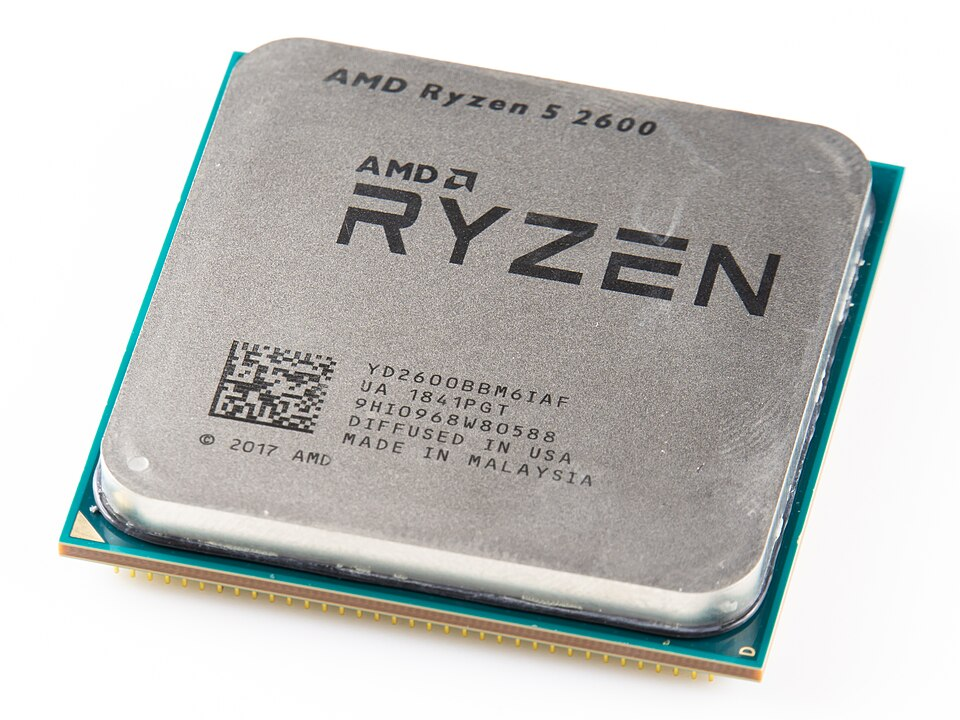
\includegraphics[width=\linewidth,height=2.7cm,keepaspectratio]{Grundlagen_Info/16_ComputerUndKodierungen/Figures/cpu.jpg}
\vskip2pt
\textbf{\scriptsize CPU}\\\tiny Prozessor (Sockel)
\column{0.24\textwidth}
\centering
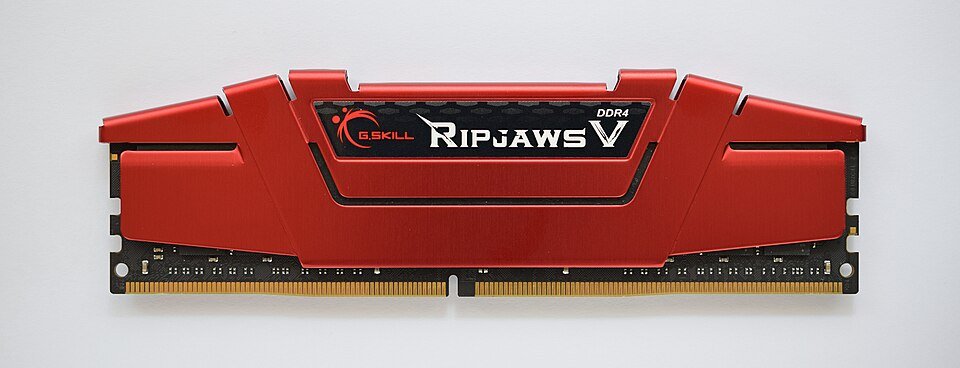
\includegraphics[width=\linewidth,height=2.7cm,keepaspectratio]{Grundlagen_Info/16_ComputerUndKodierungen/Figures/ram.jpg}
\vskip2pt
\textbf{\scriptsize RAM}\\\tiny Arbeitsspeicher
\column{0.24\textwidth}
\centering
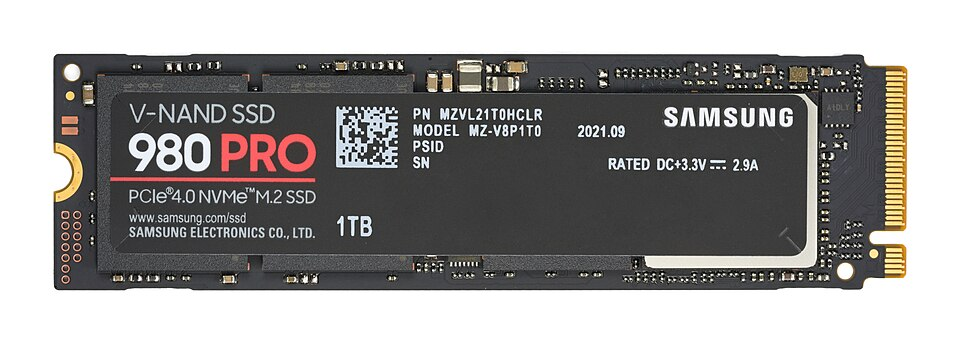
\includegraphics[width=\linewidth,height=2.7cm,keepaspectratio]{Grundlagen_Info/16_ComputerUndKodierungen/Figures/ssd.jpg}
\vskip2pt
\textbf{\scriptsize SSD}\\\tiny Massenspeicher
\column{0.24\textwidth}
\centering
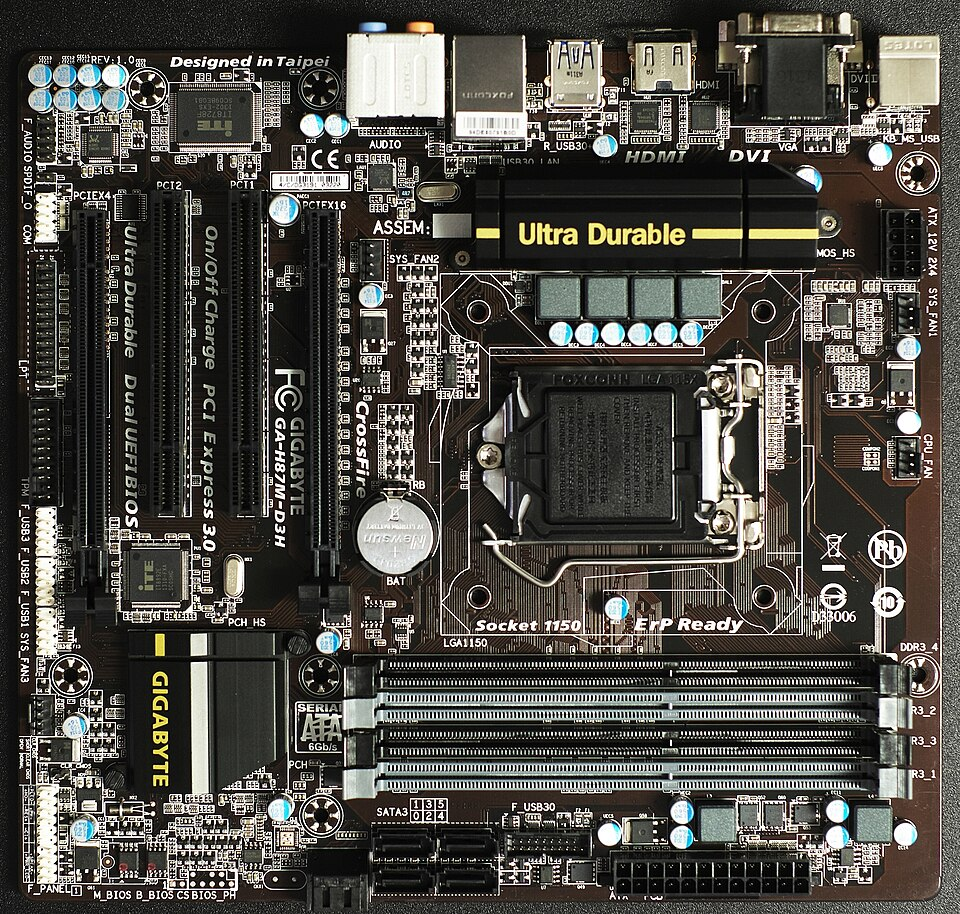
\includegraphics[width=\linewidth,height=2.7cm,keepaspectratio]{Grundlagen_Info/16_ComputerUndKodierungen/Figures/mainboard.jpg}
\vskip2pt
\textbf{\scriptsize Mainboard}\\\tiny Hauptplatine / Busse
\end{columns}
\end{frame}

\begin{frame}\FDUtitle{Warum ist das riskant?}
\begin{center}
Was könnte passieren, wenn ein fehlerhaftes Programm versehentlich seinen eigenen Programmcode überschreibt?
\end{center}
\only<2->{
\begin{center}\color{FDUteal}\bfseries Unvorhersehbares Verhalten oder Absturz -- deshalb übernimmt später das Betriebssystem den \enquote{Speicherschutz} (Lektion 12).\end{center}
}
\end{frame}

{\setbeamertemplate{footline}{\darkfootline}
\begin{frame}\sectionframe[FDUgreen]{Die CPU im Detail}{ALU, Steuerwerk, Register}
\end{frame}}

\begin{frame}\FDUtitle{ALU -- Arithmetisch-logische Einheit}
\begin{itemize}[<+->]\setlength\itemsep{7pt}
  \item Das \enquote{Rechenzentrum} der CPU
  \item Arithmetische Operationen (Addition, Subtraktion, \ldots)
  \item Logische Operationen (AND, OR, Vergleiche, \ldots)
  \item Intern: eine grosse Anzahl kombinierter Logikgatter (z.\,B.\ Volladdierer)
\end{itemize}
\end{frame}

\begin{frame}\FDUtitle{Steuerwerk \& Register}
\begin{columns}[T,onlytextwidth]
\begin{column}{.46\textwidth}
\large\bfseries\color{FDUteal}Steuerwerk
\vspace{2mm}
\normalsize
\begin{itemize}[<+->]\setlength\itemsep{5pt}
  \item Steuert den Ablauf aller Operationen
  \item Liest Befehle, interpretiert sie
  \item Gibt Steuersignale an ALU \& Co.
\end{itemize}
\end{column}
\begin{column}{.46\textwidth}
\large\bfseries\color{FDUblue}Register
\vspace{2mm}
\normalsize
\begin{itemize}[<+->]\setlength\itemsep{5pt}
  \item Sehr schnelle, winzige Zwischenspeicher
  \item Halten die aktuellen Rechenwerte
  \item Typische Grösse: 64 Bit (= 8 Byte)
\end{itemize}
\end{column}
\end{columns}
\end{frame}

\begin{frame}{Auftrag}{Kapitel 5: Von-Neumann-Architektur \& CPU}
\aufgabebox{\textbf{Aufgabe 5.1}}
\end{frame}
